\documentclass[11pt]{article}
\usepackage[margin=1in, top=1in]{geometry}
\usepackage[all]{nowidow}
\usepackage[hyperfigures=true, hidelinks, pdfhighlight=/N]{hyperref}
\usepackage[separate-uncertainty=true, group-digits=false]{siunitx}
\usepackage{graphicx,amsmath,physics,tabto,float,amssymb,pgfplots,verbatim,tcolorbox}
\usepackage{listings,xcolor,subcaption,caption,import,wrapfig,minted,biblatex}
\usepackage[version=4]{mhchem}
\usepackage[noabbrev]{cleveref}
\usepackage[british]{babel}
\newcommand{\creflastconjunction}{, and\nobreakspace}
\newcommand{\mb}[1]{\mathbf{#1}}
\numberwithin{equation}{section}
\numberwithin{figure}{section}
\numberwithin{table}{section}
\captionsetup{font=small, belowskip=0pt}
\pgfplotsset{compat=1.17}
\addbibresource{bibliography.bib}
\usemintedstyle{vs}
\definecolor{LightGray}{HTML}{eaeaea}
\setminted{framesep=2mm,bgcolor=LightGray,fontsize=\footnotesize,linenos,breaklines}
\addbibresource{bibliography.bib}

\begin{document}

\begin{center}
    {\huge Investigating the gamma-ray spectra of radiation sources 152Eu and AmBe}\\
    \vspace{0.2in}
    \textbf{KDSMIL001 | October 2022}
\end{center}


\section{Introduction}\label{sec:Introduction}
There are many sources of photon radiation naturally present in the world. Gamma-rays (roughly between \SI{0.001}{\mega\electronvolt} and \SI{10}{\mega\electronvolt}) are the highest energy and thus most dangerous form of photon radiation. For this reason, understanding where gamma-rays come from and how they interact with matter is of great importance. 

\section{Theory}\label{sec:Theory}

\subsection{Gamma-rays}\label{sec:GammaTheory}
One of the main sources of gamma-rays is from the de-excitation of nuclei. Similar to how electrons surrounding the nucleus can be excited and then emit a photon (usually an X-ray) when they de-excite, the nuclei of atoms can be excited and when they drop down to a lower energy, they emit a photon. Due to the greater mass of nuclei compared to electrons, their possible states have a much larger energy gap and thus the energy of the emitted photons is far greater. These energy levels are also very well defined, so for a given nucleus, we expect to see gamma-rays at specific, given energies. 

Unlike electrons, nuclei don't often get excited simply by an incoming photon simply because the likelihood of a gamma-ray of the right energy being in the right place is so low. For this reason, the vast majority of gamma-rays that we see come either from nuclear decays or nuclear reactions. When a radionuclide decays, it has a chance to decay to a daughter nucleus that is not in its ground state. The daughter nucleus can then de-excite by emission of a gamma-ray. The half-life of this excited state is usually on the order of picoseconds while the common radionuclides that we see in the lab have half-lives on the order of at least a few months, if not years. We can then quite confidently correlate gamma-ray emission (and thus detection) with a decay. In a similar way when nuclei gain nucleons through some nuclear process, they can also become excited and thus decay by emission of a gamma-ray. 

\subsection{Detector theory}\label{sec:DetectorTheory}
The detector used in this experiment is a NaI (Sodium Iodide) crystal scintillation detector. These detectors are designed to detect photons and work by the following principles. When a photon passes through the detector material it has 3 ways of departing its energy onto the detector. It can either be completely absorbed by an atom through photoelectric absorption (resulting in an energetic photoelectron that gets ejected from the atom), Compton scatter off an electron in the material (and send the electron flying), or pair produce an electron-positron pair. These processes all result in an electron (or positron) travelling freely through the detector material that excites other electrons in the crystal lattice. These electrons de-excite by emission of a visible light photon that is directed to the cathode of a high voltage photomultiplier tube, which turns the signal into a voltage pulse that is proportional to the energy of the initial photon.

The 3 processes which result in the free electrons have different relative cross-sections at different energies. The photoelectric effect is most dominant at low energies, dropping off as energy increases; pair production can only start at an energy of \SI{1.022}{\mega\electronvolt}, as it needs to produce an electron and positron, and only gets more dominant from that point; and Compton scattering takes over between the two. This is relevant as the 3 processes have distinct signatures when looking at the gamma-ray spectrum of some radionuclide. The photoelectric effect is effectively lossless, with all the photon's energy being transferred to the electron and thus onto the detector. Compton scattering, however, is limited by the kinematics of the situation meaning it can only ever deposit a fraction of the photon energy in one interaction. This leads to a so-called Compton continuum that begins at very low energies and stops at the Compton edge, the energy of which is related to the original photon energy by 
\begin{equation}
    E_\mathrm{Compton}=\frac{2E_\gamma^2}{m_e c^2 + 2E_\gamma}.
\end{equation}
Pair production produces an electron-positron pair. The electron is very likely to behave well and deposit all its energy, but the positron has a high likelihood of annihilating with electrons in the crystal and producing back-to-back \SI{511}{\kilo\electronvolt} photons. These photons can be absorbed again and all is good, or one or both of them could escape the detector with all their energy. Thus, for photons greater than \SI{1022}{\kilo\electronvolt} we expect to see two ``escape peaks'' at \SI{511}{\kilo\electronvolt} and \SI{1022}{\kilo\electronvolt} below the original energy. 

\section{Method}\label{sec:Method}
The apparatus was configured as in \cref{fig:Apparatus}. The detector is an NaI scintillator detector and photomultiplier tube. The preamplifier is an ORTEC model 113. The amplifier is an ORTEC model 572. The MCA is a SPECTECH UCS-30. The oscilloscope was used simply for monitoring. The HV was set to \SI{700}{\volt}.

\begin{figure}[h]
    \begin{center}
        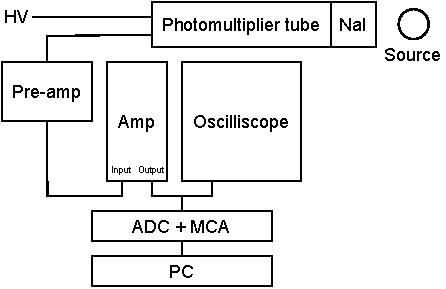
\includegraphics[width=.6\textwidth]{Plots/apparatus.pdf}
        \caption{Schematic of the set-up used in the experiment.}
        \label{fig:Apparatus}
    \end{center}
\end{figure}



energy resolution from Knoll eqn 18.1


\section{Calibration \& Energy Resolution}\label{sec:CalibrationResolution}
The radioactive sources used for calibration were \ce{^{22}Na}, \ce{^{60}Co}, and \ce{^{137}Cs}. A gamma spectrum was captured for a live time of \SI{1200}{\second} for each source. A background reading of \SI{1200}{\second} was also recorded. Two energy ranges were needed so this was done twice, reducing the gain on the amplifier for the second run in order to reach a higher energy in the highest bin of the MCA. 

For both configurations, the channel number for the centroid value of each photopeak was determined by fitting a gaussian. A scatter plot was made relating channel number to expected photopeak energy (sourced from NuDat3~\cite{nudat}) and a straight line fitted. Standard deviation on the fitted gaussians was used as uncertainty on the channel number. 

\begin{figure}[h]%
    \centering
    \begin{subfigure}[t]{.49\linewidth}
        \centering
        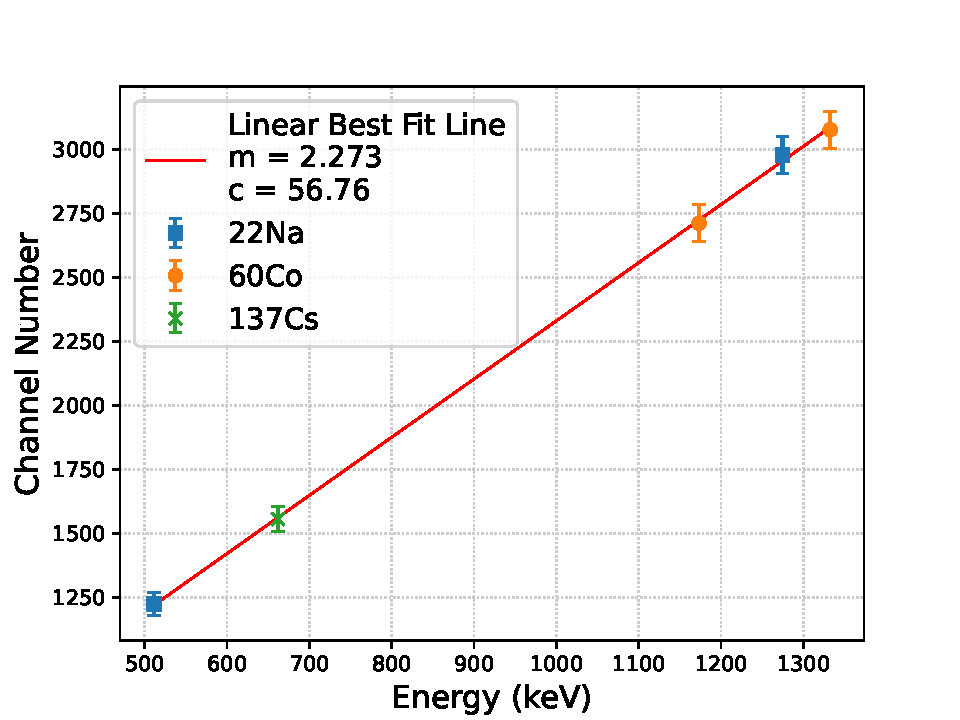
\includegraphics[width=\linewidth]{Plots/low_calibration.pdf}
        \caption{Scatter plot and fitted line for the low energy calibration. The largest energy resolvable with this calibration was \SI{1776}{\kilo\electronvolt}.}
        \label{fig:low_calibration}
    \end{subfigure}
    \hfill
    \begin{subfigure}[t]{.49\linewidth}
        \centering
        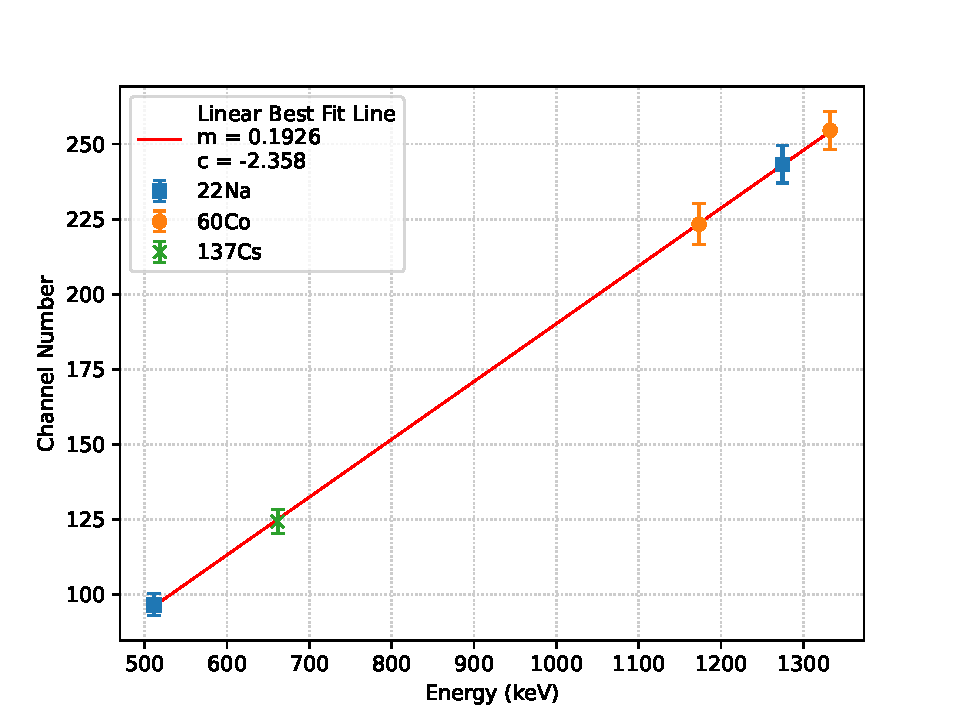
\includegraphics[width=\linewidth]{Plots/high_calibration.pdf}
        \caption{Scatter plot and fitted line for the high energy calibration. The largest energy resolvable with this calibration was \SI{5330}{\kilo\electronvolt}.}
        \label{fig:high_calibration}
    \end{subfigure}
\caption{}
\label{fig:calibration}
\end{figure}

To find the energy resolution, the primary photopeaks of the calibration sources were used. Using the standard deviation found earlier, the FWHM maximum was found with $FWHM=2\sqrt{2\ln(2)}\sigma$ and the energy resolution found from \cite[Fig. 4.5]{Knoll}:

\begin{equation}
    R=\frac{FWHM}{H_0}
    \label{eqn:EnergyResolution}
\end{equation}
where $H_0$ is the mean of the gaussian. Taking the mean of the 5 values, a resolution of 6.855\% was found. This means that for a photon of a given energy $E$, there will be a range with width $6.855\%\times E$ around that energy for which a photon of a different energy to the original will not be resolvable. 

\section{125Eu}\label{sec:Eu}


\section{AmBe}\label{sec:AmBe}

\subsection{AmBe Theory}
The Americium-Beryllium (AmBe) source is a neutron source that works of the principle of creating 

\section{Conclusion}\label{sec:Conclusion}

\newpage
\printbibliography

\end{document}